\documentclass{article}
\usepackage[margin=1.0in]{geometry} % smaller margin for document
\usepackage[margin=.7in]{caption} % little more margin for captions to make look nice
\usepackage{graphicx}
\usepackage[counterclockwise, figuresleft]{rotating} % get the heatmap rotated correctly

\title{The effect of pipeline-collection-diversity on performance}

\author{Sean Carver @ Data Machines Corporation}

\begin{document}

\maketitle

\abstract{Do performers who submit \emph{diverse} collections of
  pipelines tend to perform better than those who submit less diverse
  collections of pipelines? The answer for the Winter 2020 evaluation is effectively no. While there does exist statistically significant effect of increased diversity on increased score, the effect size is trivial. Thus, it seems that less diverse collections of pipelines, i.e. those that focus more on hyperparameter tuning, can be as effective as those that explore a greater diversity and/or ordering of primitives. }

\section{Introduction}
In section \ref{sec:measures}, \emph{Measures of Diversity}, we define
several measures of the diversity within a collection of three or more
pipelines. In section \ref{sec:glance}, \emph{Results at a Glance}, we present a
heat map showing briefly the (weak) connection between diversity and
performance. In section \ref{sec:quantifying}, \emph{Quantifying the Effect of Diversity}, we report on regression results which point to the measurable, though substantively trivial, effect of diversity on score. In a final section \ref{sec:visualization}, \emph{Visualizing Collections} we show a  visualization of collections of
pipelines for a problem together with a multiple alignment, for context.

\section{Measures of Diversity}
\label{sec:measures}
Before we can define \emph{diversity} of a collection of (say 3 to 20)
pipelines, we first need to define the distance between a pair of pipelines.
We choose the Levenshtein edit distance as this measure between two
pipelines.  Specifically, we first express the pipelines as sequences
of primitives, where primitives are written as ``letters'' in a large
alphabet.  The software we use accommodates all D3M primitives with
two-letter pairs, each pair representing a single token
(primitive) of the alphabet.  The Levenshtein edit distance is the
minimum number of substitutions, insertions and/or deletions needed to
bring one sequence to coincide with the other.  This measure satisfies
the axioms for a distance.

But \emph{distance} involves just two pipelines; \emph{diversity} measures variation
among a collection of three or more pipelines.  We tried several
alternatives for quantifying diversity.  The most well-behaved
measures (i.e.\ the ones that behave most closely to our expectations
on synthetic data) were vector norms where the vector components were
the Levenshtein distances for all possible unordered pairs of
pipelines in the collection.

More precisely, we used $l_p$ norms where $p$ was a parameter varying
between 1 and $\infty$.  The different norms measure slightly different
quantities.  At the extreme, the $l_\infty$ norm (maximum
edit-distance component) is large when there is at least one pair of
pipelines at great distance, regardless of the positions (great or
small) of the other as-close or closer distances.  On the other hand,
the $l_1$ norm (sum of the edit-distance components) can still be
relatively large if there are many pairs pipelines at moderate
distance, even though there is no pair at great distance.  We point
out that the choice the different norms can sometimes matter: we have
noted that the choice can order sets of collections---synthetic or
real---differently in terms of diversity.

%Note that absolute values found in textbook definitions of the $l_p$
%norm:
%$$l_p([v_1,\dots,v_n]) = \sqrt[p]{|v_1|^p + \dots + |v_n|^p}$$ remain
%unnecessary because all distances (e.g.\ the Levenshtein edit distance
%components of $v$) must be non-negative by the properties of distance.

In the $l_p$ norm, what value for the parameter $p$ do we pick?  If
you are using only one measure of diversity, we recommend the $l_2$
norm as a nice tradeoff between the two extremes.  That said, it is
more informative to report two or more measures of diversity, in which
case $l_1$ and $l_\infty$ should be preferred because they are most
independent.

\section{Results at a Glance}
\label{sec:glance}
Figure \ref{fig:heatmap} shows the diversity of performer pipeline submissions by problem type. The color-coding indicates diversity, with purple colors indicating small $l_2$ edit distance norms, trending towards yellow colors indicating larger $l_2$ edit distance norms.The number of asterisks in each cell captures the count of times a pipeline in that performer-category was the best (or tied). For instance, in the second row of the first column, UCB twice had the best-performing pipeline on a dataset in the binary\_classification problem category. Overall, the figure suggests (and we quantify below) a very small but measurable effect of diversity.

% the [h] asks LaTeX to keep the image Here
\begin{sidewaysfigure}
% typically cenetered
\centering
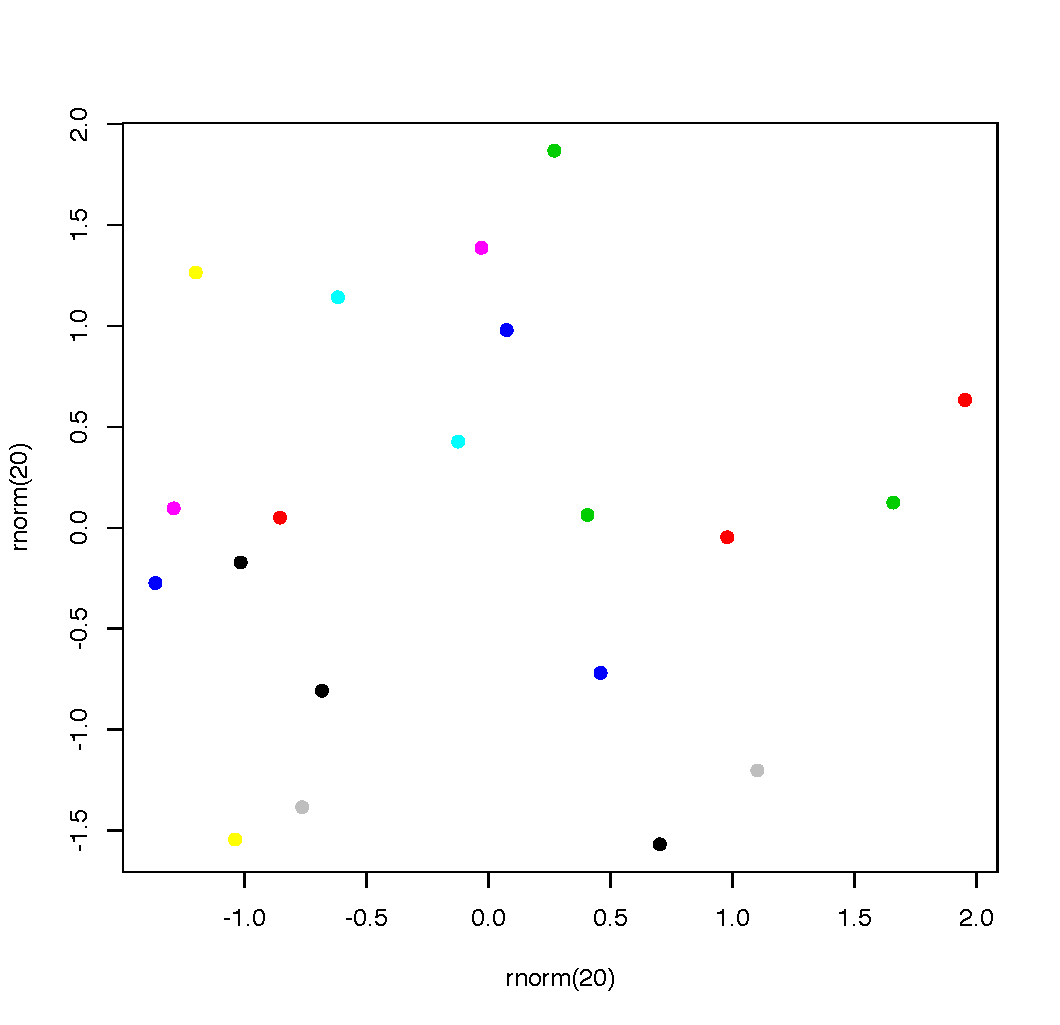
\includegraphics[scale=1.3]{heatmap.pdf}
\caption{Heat map of $l_2$ diversity see section ``Measures of
  Diversity'' for a discussion of this and other measures we use to
  quantify diversity.  The horizontal axis is the problem category and
  the vertical axis is performer for the Winter 2020 evaluation.  The
  number of asterisks in each cell is the number of problem instances
  in the corresponding category-performer which was the best (or tied
  for best) performing pipeline for any problem.  There were 37 ties
  (including multi-way ties), corresponding to an additional 37
  asterisks in the figure beyond the total number of 103 problems.}
\label{fig:heatmap}
\end{sidewaysfigure}

\section{Quantifying the Effect of Diversity}
\label{sec:quantifying}
We use regression-based methods to quantify the effect of diversity on score. This analysis is complicated by several factors, which we address by various, overlapping methodological choices. Overall, our goal is to specify predictive models of score on the bases of the $l_1$ and $l_\infty$ norms, as well as the number of pipelines submitted. Our unit of analysis is the collection of pipelines submitted by a performer, which features diversity measures mentioned, a count, and the score obtained by its best member. We group these by problem-types (e.g. ``binary classification'') for analysis. The diversity measures and scores are not comparable across problems, or problem types; thus, we move to measuring all predictors and scores on a per-problem-type z-score basis. 

Below, we report on XXX classes of statistical models. In the first, we group all problem types together for analysis in a ``complete pooling'' model; see  MODEL 1. We can see that INTERPRET RESULTS. We ran a model including fixed effects for problem type, and saw no change in our key predictors. We evaluated the possibility of multicollinearty by running PCA over our predictors and using the first principal component as an omnibus measure of diversity, and found (whatever we found; see MODEL 2).


\section{Visualizing Collections}
\label{sec:visualization}
In this final section, we show a cartoon visualization of collections
of pipelines for a problem together with a multiple alignment.

\end{document}


  
